\documentclass{standalone}
\usepackage{xcolor}
\usepackage{verbatim}
\usepackage[T1]{fontenc}
\usepackage{graphics}
\usepackage{hyperref}
\newcommand{\code}[1]{\texttt{#1}}
\newcommand{\R}{R}
\newcommand{\pkg}[1]{#1}
\newcommand{\CRANpkg}[1]{\pkg{#1}}%
\newcommand{\BIOpkg}[1]{\pkg{#1}}
\usepackage{amsmath,amssymb,array}
\usepackage{booktabs}
\usepackage{subcaption}
\usepackage{tikz}  
\usetikzlibrary{shapes.geometric, arrows.meta, positioning}

\begin{document}
\nopagecolor
\centering

\label{fig:relms-workflow-general-weighted}
\vspace{0.5em}
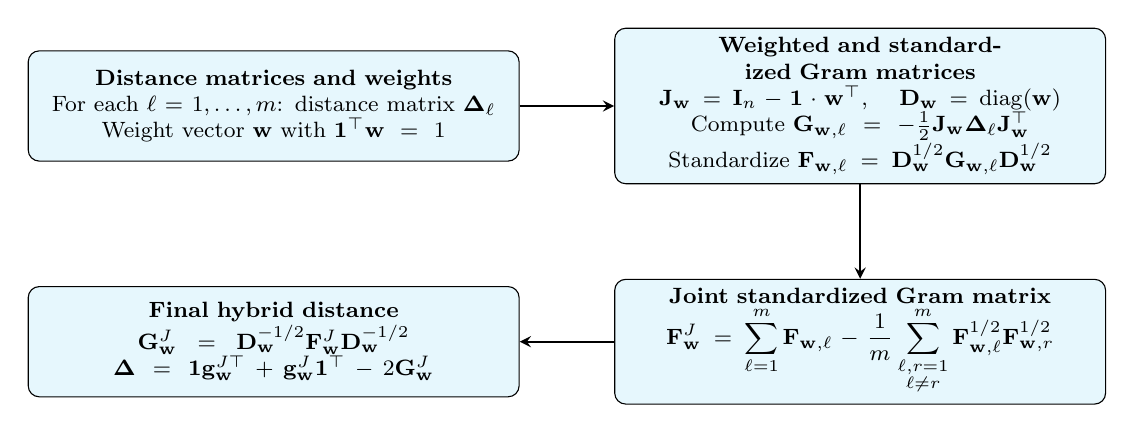
\begin{tikzpicture}[node distance=1.2cm and 1.2cm, >=stealth]
\tikzset{
  box/.style={rectangle, draw, text width=6cm, align=center, rounded corners,
              minimum height=1.4cm, fill=cyan!10, font=\footnotesize},
  arrow/.style={->, thick}
}
\node[box] (A) {
 \textbf{Distance matrices and weights} \\
  For each $\ell = 1,\dots,m$: distance matrix $\mathbf{\Delta}_\ell$ \\
  Weight vector $\mathbf{w}$ with $\mathbf{1}^\top \mathbf{w} = 1$
};
\node[box, right=of A] (B) {
  \textbf{Weighted and standardized Gram matrices} \\
  $\mathbf{J}_\mathbf{w} = \mathbf{I}_n - \mathbf{1}\cdot \mathbf{w}^\top$, \quad $\mathbf{D}_\mathbf{w} = \mathrm{diag}(\mathbf{w})$ \\
  Compute $\mathbf{G}_{\mathbf{w},\ell} = -\frac{1}{2}\mathbf{J}_\mathbf{w} \mathbf{\Delta}_\ell \mathbf{J}_\mathbf{w}^\top$ \\
 Standardize $\mathbf{F}_{\mathbf{w},\ell} = \mathbf{D}_\mathbf{w}^{1/2}\mathbf{G}_{\mathbf{w},\ell}\mathbf{D}_\mathbf{w}^{1/2}$
};
\node[box, below=of B] (C) {
  \textbf{Joint standardized Gram matrix} \\
  $\displaystyle
  \mathbf{F}_\mathbf{w}^J = \sum_{\ell=1}^{m}\mathbf{F}_{\mathbf{w},\ell} - \frac{1}{m}\sum_{\substack{\ell,r=1\\\ell\neq r}}^{m}\mathbf{F}_{\mathbf{w},\ell}^{1/2}\mathbf{F}_{\mathbf{w},r}^{1/2}$
};
\node[box, left=of C] (D) {
  \textbf{Final hybrid distance} \\
  $\mathbf{G}_\mathbf{w}^J = \mathbf{D}_\mathbf{w}^{-1/2}\mathbf{F}_\mathbf{w}^J\mathbf{D}_\mathbf{w}^{-1/2}$ \\
  $\mathbf{\Delta} = \mathbf{1}\mathbf{g}_\mathbf{w}^{J\top} + \mathbf{g}_\mathbf{w}^J\mathbf{1}^\top - 2\mathbf{G}_\mathbf{w}^J$
};
\draw[arrow] (A) -- (B);
\draw[arrow] (B) -- (C);
\draw[arrow] (C) -- (D);
\end{tikzpicture}
\end{document}
